% document-level settings
\documentclass[border=0.125cm]{standalone}
\usepackage{tikz}
\usepackage{amssymb}
\usetikzlibrary{positioning}

\begin{document}

% re-usable tikzset
\tikzset{
  every neuron/.style={
    circle,
    draw,
    minimum size=1cm
  },
  neuron missing/.style={
    draw=none, 
    scale=2,
    fill=none,
    text height=0.333cm,
    execute at begin node=\color{black}$\vdots$
  },
}

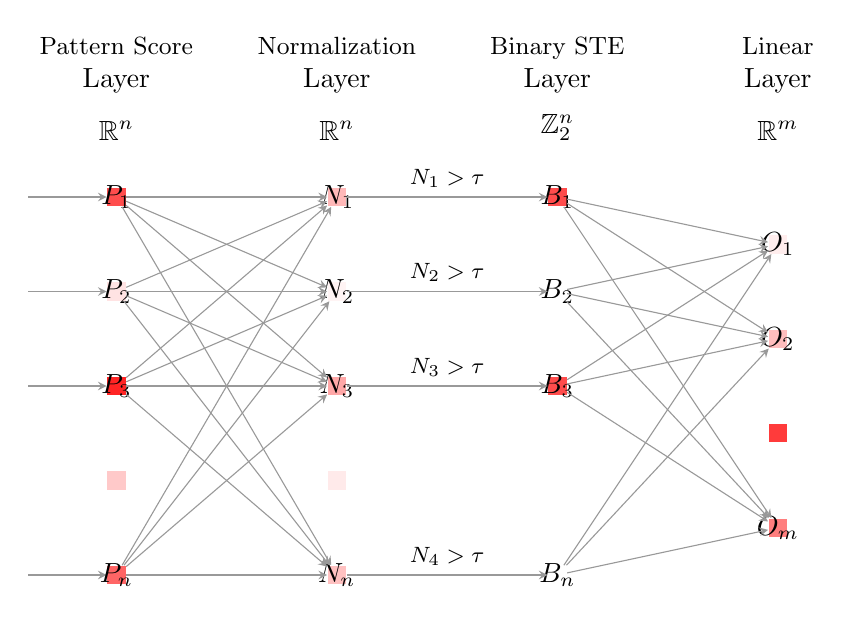
\begin{tikzpicture}[x=1.4cm, y=1.2cm, >=stealth]

  % create and distribute neurons
  {
    % set random seed for color generation 
    \pgfmathsetseed{1}    
    \foreach \m/\l [count=\y] in {1,2,3,missing,4}{
      \pgfmathparse{100*rnd}
      \edef\tmp{\pgfmathresult}
      \node [every neuron/.try, fill=red!\tmp, neuron \m/.try] (score-\m) at (0,2.5-\y) {};
    }

    % set random seed for color generation 
    \pgfmathsetseed{1}
    \foreach \m [count=\y] in {1,2,3,missing,4}{
      \pgfmathparse{40*rnd}
      \edef\tmp{\pgfmathresult}
      \node [every neuron/.try, fill=red!\tmp, neuron \m/.try ] (layernorm-\m) at (2,2.5-\y) {};
    }
    
    \foreach \m [count=\y] in {1,2,3,missing,4}{
      \ifnum \y=1
      \node [every neuron/.try, fill=red!70!white, neuron \m/.try ] (ste-\m) at (4,2.5-\y) {};
      \else
      \ifnum \y=3
      \node [every neuron/.try, fill=red!70!white, neuron \m/.try ] (ste-\m) at (4,2.5-\y) {};
      \else
      \node [every neuron/.try, neuron \m/.try ] (ste-\m) at (4,2.5-\y) {};
      \fi
      \fi
    }

    % set random seed for color generation 
    \pgfmathsetseed{3}
    \foreach \m [count=\y] in {1,2,missing,3}{
      \pgfmathparse{80*rnd}
      \edef\tmp{\pgfmathresult}
      \node [every neuron/.try, fill=red!\tmp, neuron \m/.try ] (output-\m) at (6,2-\y) {};
    }
  }
  
  % label neurons and draw border arrows
  {
    \foreach \l [count=\i] in {1,2,3,n}{
      \draw [<-, black!40!white] (score-\i) -- ++(-0.8,0) {};    
      \node at (score-\i) {$P_\l$};
    }
    
    \foreach \l [count=\i] in {1,2,3,n}
    \node at (layernorm-\i) {$N_\l$};

    \foreach \l [count=\i] in {1,2,3,n}{
      \node at (ste-\i) {$B_\l$};
    }

    \foreach \l [count=\i] in {1,2,m}
    \node at (output-\i) {$O_\l$};
  }

  % draw inter-connecting arrows
  {
    \foreach \i in {1,...,4}
    \foreach \j in {1,...,4}
    \draw [->, black!40!white] (score-\i) -- (layernorm-\j);

    \foreach \i in {1,...,4}
    \draw [->, black!40!white] (layernorm-\i) -- (ste-\i) node [above, midway, black] {\footnotesize $N_\i > \tau$} ;

    \foreach \i in {1,...,4}
    \foreach \j in {1,...,3}
    \draw [->, black!40!white] (ste-\i) -- (output-\j);
    
    \foreach \l [count=\x from 0] in {Pattern Score, Normalization, Binary STE, Linear}
    \node [align=center, above] at (\x*2,2.5) {\small \l \\ Layer};

    \foreach \l [count=\x from 0] in {$\mathbb{R}^n$, $\mathbb{R}^n$,
      $\mathbb{Z}_2^n$, $\mathbb{R}^m$}{
      \node [align=center, above] at (\x*2,2) {\l};
    }
  }
  
\end{tikzpicture}

\end{document}